\documentclass[twoside]{article}
\hoffset-2.5cm
\voffset-2.5cm
\textwidth16cm
\textheight26cm
\oddsidemargin2.4cm
\evensidemargin2.4cm
\usepackage{graphicx}
 \usepackage{makeidx}
 \usepackage{html}
\usepackage{lscape}
\usepackage{amssymb}
\usepackage{amsbsy}
\usepackage{xcolor}
%\usepackage[utf8]{inputenc}
%\usepackage{amsmath}
%\usepackage{empheq}
%\usepackage{bbm}
%\usepackage{dsfont}
\usepackage{hyperref} 
\makeindex
\newcommand\mybar[1][black]{\begingroup\color{#1}\kern1pt\rule[-\dp\strutbox]{1pt}{\baselineskip}\kern1pt\endgroup}
\newcommand{\highlight}[1]{\colorbox{red!10}{$\displaystyle#1$}}
\newcommand{\m}[1]{\overline{#1}}
\newcommand{\M}[1]{\underline{#1}}
\newcommand{\mbf}[1]{\mathbf #1}
\newcommand{\V}[1]{ \stackrel{=}{\mathbf #1}}
\newcommand{\B}[1]{#1}
\newcommand{\prg}{\sl}
\newcommand{\use}[1]{\vspace{0.5cm} Usage: {\prg{ #1}} \vspace{0.5cm}}
\newcommand{\bra}[1]{\langle #1|}
\newcommand{\ket}[1]{|#1\rangle}
\newcommand{\threej}[2]{\left( \begin{array}{ccc} #1 \\ #2 \end{array} \right)}
\newcommand{\sixj}[2]{\left\{ \begin{array}{ccc} #1 \\ #2 \end{array} \right\}}
\newcommand{\hili}[1]{{#1}}
\newcommand{\hl}[1]{{#1}}
\newcommand{\text}[1]{{\rm #1}}
\newcommand{\Bell}{\ensuremath{\boldsymbol\ell}}
\newcommand{\bm}[1]{\boldsymbol #1}
\newcommand{\Trace}[1]{\rm Tr \{ #1 \} }
\newcommand{\oo}{Orlando }
\newcommand{\OO}{\hspace*{-1cm} ORLANDO: }
\newcommand{\ee}{Ewald }
\newcommand{\EE}{\hspace*{-1cm} EWALD: }
\newcommand{\pp}{Simplicius }
\newcommand{\PP}{\hspace*{-1cm} SIMPLICIUS: }
\setlength{\parindent}{0em}
\begin{document}


 \title{ 

\includegraphics[bb=0 0 413 289,angle=0,height=90pt]{figsrc/headerL.jpg}
\includegraphics[bb=0 0 389 282,angle=20,height=140pt]{figsrc/mcphase_logo.jpg}

\includegraphics[bb=0 0 413 289,angle=0,height=90pt]{figsrc/headerR.jpg}

% {\Huge \bf \em McPhase} \\
 \vspace{1cm} 
{\bf   USERS MANUAL}\\
  \vspace{1cm} 
{\em  Workshops available at the McPhase homepage }

\href{https://mcphase.github.io/webpage/}{mcphase.github.io/webpage/} 

{We offer workshops with  few participants online or in
 a relaxed atmosphere in Venice, Italy, a city without the stress of cars.}

%\vspace{1cm}

\includegraphics[bb=0 0 700 180,angle=0, width=0.9\textwidth]{figsrc/McPhaseVenice.jpg}
%\vspace{1cm}
}

\date {
\vspace{1cm} 
       mcphas 5.7 experimental code - do not use!
mcdisp 5.7 experimental code - do not use!
mcdiff 5.7 experimental code - do not use!
5.7 experimental code - do not use!

 %      \vspace{1cm}
       \today}
%\begin{center}
%\end{center}

\author{M. Rotter\thanks{Independent international Scientific Consultant, email: mcphase@icloud.com}, 
\and Duc Manh Le \thanks{Dept. Physics and Astronomy, Seoul National University, Seoul 151-742, Korea}
\and Joachim Keller \thanks{Universit\"at Regensburg}
\and Till Hoffmann  \thanks{University of Oxford, Physics Department, Clarendon Laboratory, Parks Road, Oxford, UK},
\and P. Fabi n\'e Hoffmann\thanks{Forschungszentrum J\"ulich, D-52425 J\"ulich, Germany},
\and S. Rotter \thanks{Wien, Austria}
}


\maketitle
\clearpage
\pagestyle{myheadings}
\markboth{\hfill 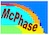
\includegraphics[angle=20,height=20pt,bb=0 0  49 35]{../mcphas_logo1.jpg} }
          {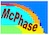
\includegraphics[angle=20,height=20pt,bb=0 0 49 35]{../mcphas_logo1.jpg} \hfill}

\subsection*{To the discreet Reader}

400 years ago it was in the peaceful lagoon of Venice, where Galileo Galilei found bamboo
 and the first man to fabricate transparent glass so he could build a telescope.  
His telescope soon provided evidence for new models of the solar system in contrast
to the AI, the Aristotelian Intelligence. In his words "In questions of science, 
the authority of a thousand is not worth the humble reasoning of a single individual."

Today it is in the peaceful lagoon of Venice, where at the beginning of the year gathers a small
group of scientists. Circumvented by the floating water of the lagoon they
 build a new kind of simulation suite for models of the solid state.
The concept is in contrast to the wide spread focus on purely electronic properties
promoted by many cardinals of science. 

In this manual, frequently there appear three characters in conversations. The 
first one is \oo, who is appassionate about creating high magnetic fields.
He is of hot temperament and loves basic science which can be applied to 
technical devices. \oo  does not like complicated formulas but is willing
to collaborate with theoreticians to get a better understanding of material properties.
The second character is \ee - he is, in contrast to \oo in love with
formulas and mathematical treatises. He is extremely accurate and 
if we let him alone write this book, we will
end up with a large pile of paper and it will be hard to find out where to
look up what. The third person the reader will meet is \pp, 
 he is  simple minded and a
strong personality who will not tolerate any other opinion. He tries to
control the direction of activities such as to promote his interest. His 
interest is mainly that of controlling the activities by evaluating the work
which is done by others. 

By means of their lively discussions we hope to immerse
 the appreciated reader into the lagoon of ideas which penetrates
 the models of solid matter.








\subsection*{Acknowledgements}

We would like to thank colleagues who generously agreed to read sections of the draft version
of the text; their comments helped to improve the text substantially. We are particularly indebted to
Ulrike Witte, Jane Brown, Michael Loewenhaupt, Jens Jensen, Andreas Kreyssig, Enrico Faulhaber,
Jesus Blanco, Maurits Haverkort, Andrea Severing,
Andreas Doenni, Hideoki Kitazawa, Reinhard Kremer, Arata Tanaka, N. Kl\"uver, Herwig Michor,
Michael Banks, Nan Tang, Lucian G Pascut, Mathias Doerr, Roland Schedler, Adroja Devashibhai, Danny Milosavljevic,
Tobias Weber
 and Andrew Boothroyd for their help and inspiring comments.

Furthermore, we thank the participants of McPhase Workshops for installing and
testing the new McPhase software suite before the official release:

\begin{description}
\item[McPhase 6.0]
   2026: Victor Mecoli, Tobias Weber, Zumair Muhammed, Yash Rajesh Tijare, 
   2025: Sungkyun Choi, Justus Grumbach
\item[McPhase 5.6]
   2024: Herwig Michor, Danny Milosavljevic, Juanjuan Liu, Fanjun Xu, 
      Zhentao Wang, Padraig Maderson, Justus Grumbach, Alexander Komarek
   2023: Stephan Geprägs, Fei Li, Mocabber Hossain
\item[McPhase 5.5]
   2023: Justus Grumbach, Christoph Herb, The Anh, Sungkyun Choi, Gideok Kim, Pikesh Pal, Nan Tang,
   2022: Yiqing Gu, José Abraham Hernández, Lazar Kish, Chennan Wang, Abhisek Bandyopadhyay
\item[McPhase 5.4]
   2022: Mahmoud Deeb, Shovan Dan, Rajesh Tripathi, Chennan Wang, Alexander Komarek, 
        Devashibhai T Adroja, Jose Abraham Hernandez, Jorge Lago, Lorenzo Celiberti, Dario Fiore Mosca,
        Michal Stekiel,
   2021: Christian Wessler, Mahmoud Deeb, Chennan Wang
\item[McPhase 5.3]
   2016: Jiang Xiaoming
\item[McPhase 5.2]
   2015: Ernst Bauer, Herwig Michor, Karl Sandeman, Alexander Komarek, Karina Bulgakova,
         Soner Özcan
   2014: G. E. Granroth, S. Campbell, 
\item[McPhase 5.0]
   2012: Martin Boehm, Mark H. Johnson, Jesus A. Blanco, Hideoki Kitazawa
\item[McPhase 4.6]
   2011: Devishibhai Adroja, Pablo Alvarez Alonso, Joan Amaral, Ernst Bauer,
         Joao Filipe Horta Belo da Silva, Jesus A Blanco, Andrew Boothroyd,
         Cristina Echevarvia Bonet, Belen Fernandez Alfonso, Lucas Fernandez Selvane,
         Albert Furrer, Abel Garzia Saiz, Christoph Geibel, Pedro Gorria Korres,
         Thomas Gruner, Ariane Haase, Jens Jensen, Mark Johnson, Romi Kaur, Cornelius Krellner,
         Bella Lake, Duc Manh Le, Haifeng Li, Stephen Lovesey, Michael Loewenhaupt,
         Karl Anton Lorenzer, Javier Luzon Marco, Luigi Paolasini, Toby Perring,
         Carmen Pique Rami, Natalia Rinaldi Montes, Angel Rodriguez Fernandez,
         Lucia Steinke, Subakti Subakti, Peter Thamlmeier, Linda Udby, Helen Walker,
         Yinguo Xiao, Geresi Zsolt
\end{description}



The authors thank the FWF, Royal Society and the EPSRC.
We thank the authors of Cfield, Powls, FullProf, Spectre, Amos and XTLS, output 
of these programs has been used to test McPhase. 

Without the enthusiastic support of the neutron scattering 
community this program would not have come into existence. 

\section*{What is New ?}

\subsection*{ ... in version 6.0 ...}
\begin{itemize}
\item    External Stress / Pressure
\item    Electric Field and orientational electrical Polarisation
\item    Monte Carlo Metropolis algorithm
\item    input files can contain variables and expressions such as Dz2=sqrt(2)*Dx2
\item    {\prg McPhaseExplorer} Button for opening the Manual  
\item    {\prg mcphas.ini}: flexible user defined output columns can be defined,
          Magnetic and Electric Field can be input in euclidean coordinates or as components along crystal axis,
          parameter repeat to control action if no convergence is achieved in mean field loop
\item    {\prg cif2mcphas} atomic coordinates may contain references to previous atoms x y z, e.g. O1x
\item    {\prg ic1ion} operators -  bug removed for imaginary Tkq (i.e. q<2) in expectation value calc in ic1ion 5.6 
\item    {\prg reduce\_unitcell} extended: for negative coefficient (+--) the sipf files will be overwritten
         with CHARGE replaced by distributed charge - useful for problems with electric polarisation calculations
\item    {\prg mcdisp} output files:  qom dsigma disgma.tot file have different format now (number of columns increased by one)
\item   {\prg singleion} options  introduced for dynamical and static susceptibility 
\item   {\prg makenn}: new options -rkkynest -djdeps1-6
\item    {\prg display}: option -vlines -hlines for vertical and horizontal guide to the eye lines
\item    {\prg mctest} - to test correct function of McPhase, cd  demo  and type {\prg mctest test*.bat }
\end{itemize}

\subsection*{ ... in version 5.6 ...}
\begin{itemize}
\item {\prg mcphas}
\begin{itemize}\item introduced self consistent treatment of exchange striction, see section \ref{JT}
 \item bugs removed: fecalc evalfe was not full multithreading, ic1ion and icf1ion cfp were buggy
 \item introduced experimental error in {\prg fit/mcphas.fum} for calculation of sta
            and allow for fitting of any quantity in {\prg mcphas.fum}
\end{itemize}
\item {\prg singleion} option -Tsteps -Hsteps -v introduced to allow simple loops with high speed 
\item {\prg pointc}: a standard deviation sta of calculated  to input cf parameters can be calculated (option -s)
\item {\prg fform} extended, option -t to format year month day hour min second into timestamp in seconds
\item {\prg getvalue} improved to do interpolation, too (dx=0)
\item  check of righthandedness of primitive lattice in reading {\prg mcphas.j} introduced
\item {\prg display\_density, densplt} enabled to read exchange field components from command line
\item {\prg cif2mcphas} reading of atomic positions extended to be able to put something such as
         \begin{verbatim}(C1+Tm2)/2 (C1+Tm2)/2 (C1+Tm2)/2\end{verbatim} for a position instead of 0.253(23) 0.423  0.5, 
option -nm (nonmagnetic) introduced to force nonmagnetic atoms
\item {\prg reduce\_unitcell}: check if atoms are in primitive unit cell, if not
         move them there, option -delatoms introduced to allow to delete atoms from {\prg mcphas.j}
\item TmNiC$_2$ example created, using electron point charges on bondings
         and solving linear equation system to calculate some point charges
         given $B_2^0$ and $B_2^2$ from high T expansion of inverse magnetic susceptibility
\item {\prg makenn} 
revised to make possible exchange striction calculations using option -djdx -djdy -djdz,
bug in elastic constants formula found and corrected 
\item           {\prg  display }: adapted to enable display of error bars 
\item            option -r in {\prg simannfit}
\end{itemize}


\subsection*{ \dots in version 5.5 \dots}
\begin{itemize}
\item {\prg ic1ion \& icf1ion \& mcdiff.in file format for} $\langle \mbf S \rangle$
and  $\langle \mbf L \rangle$ - !!  Operator sequence changed to Sa Sb Sc La Lb Lc !! 
(was Sa La Sb Lb Sc Lc)
\item   mcphas got an option -doeps for magnetostrictive strain calculation using parameters
calculated e.g. by makenn -cfph 
\item  there are more examples using cf-phonon interaction
\item module phonon: umax restrictino in module phonon done by 
u= umax * tanh (u/umax) ... this avoids uniform shifts of the crystal 
\item {\prg makenn} option -bvk extended to generate a sample bvk constants table 
\item anisotropy $H=D_{x4} S_x^4 +D_{y4} S_y^4 +D_{z4} S_x^4$ introduced in module {\prg so1ion}
\item made {\prg mcphaseexplorer} compatible with java 1.8.0 and java 17 at the 
           same time (see batch mpe for linux for options) 
\item {\prg cif2mcphas} changed to put phonon module for sipf files which are nonmagnetic
\item  mcphas.xyt outputs periodicity of supercell
\item {\prg spins} changed to produce for option -f spins\_prim.jvx graphics output
\item  {\prg spinsfromq} phases correctly introduced for double and triple q structure
\end{itemize}

\subsection*{ \dots in version 5.4 \dots}
\begin{itemize}
\item    {\prg bcfph} and a DMD method for Crystal Field - Phonon interaction
\item  {\prg makenn} option for Dzyalosinsky Moriya interaction created
\item .trs file format changed to include number of initial and final level
\item   {\prg powdermagnon} sampling q dependence improved
\item option -read introduced to {\prg mcphas}
\item   program {\prg substitute} option -f introduced
\item   Slatec removed from PDL routines to make installation easier
\item {\prg cpso1ion} bug (for more than 10 levels) found and removed
\item bug in {\prg makenn} options ignore\_neihgbours\_behind=1 and bvk found and removed
\end{itemize}



\newpage

\tableofcontents

\clearpage

\section{How To ... ? }
\input{../tutorial/howto.txt}

\section{Frequently asked Questions}
\input{../frequently_asked_questions.txt}

\clearpage
\section{Introduction}

\OO How nice to meet you here in Venice, \ee - 
I have some exciting new magnetostriction data in ultrahigh fields which we
are trying to understand !

\EE The pleasure is on my side - I am always impressed, how much effort you
make to do such experiments. Maybe looking into 
{\prg McPhase} can help to unterstand your data - {\prg McPhase}
  is a program package designed to calculate 
properties of a magnetic system with localised magnetic moments
given the crystal field and/or the
exchange interaction constants.

\PP Hi, do tell me, what can you do with that program ?

\EE For rare earth ions {\prg McPhase} is based on the Hamiltonian of the standard model
of rare earth magnetism~\cite{jensen91-1}.
\footnote{The Hamiltonian of the standard model of rare earth magnetism 
is described in section~\ref{hamiltonian}.}
Alternatively, a more complex Hamiltonian can be used which includes
all terms in intermediate coupling - this is important for transition metal
and actinide ions.

\PP I hope you know, that actinides are forbidden in my institute ! 
I am interested in exotic matter, this is important - so what can you study ?

\EE By means of magnetoelastic interactions 
the interplay of lattice and magnetism can be studied. Properties 
to be calculated are magnetic moments, electric polarisation, strain  and
excitations under magnetic and electric fields and stress/pressure.

\OO Indeed ? So can we do a quick calculation to understand better my
new experimental high field data of magnetisation and magnetostriction. My
student is trying really hard to set up something for pressure experiments too, it
would be nice to have some prediction from theory !

\begin{figure}[hb]\begin{center}
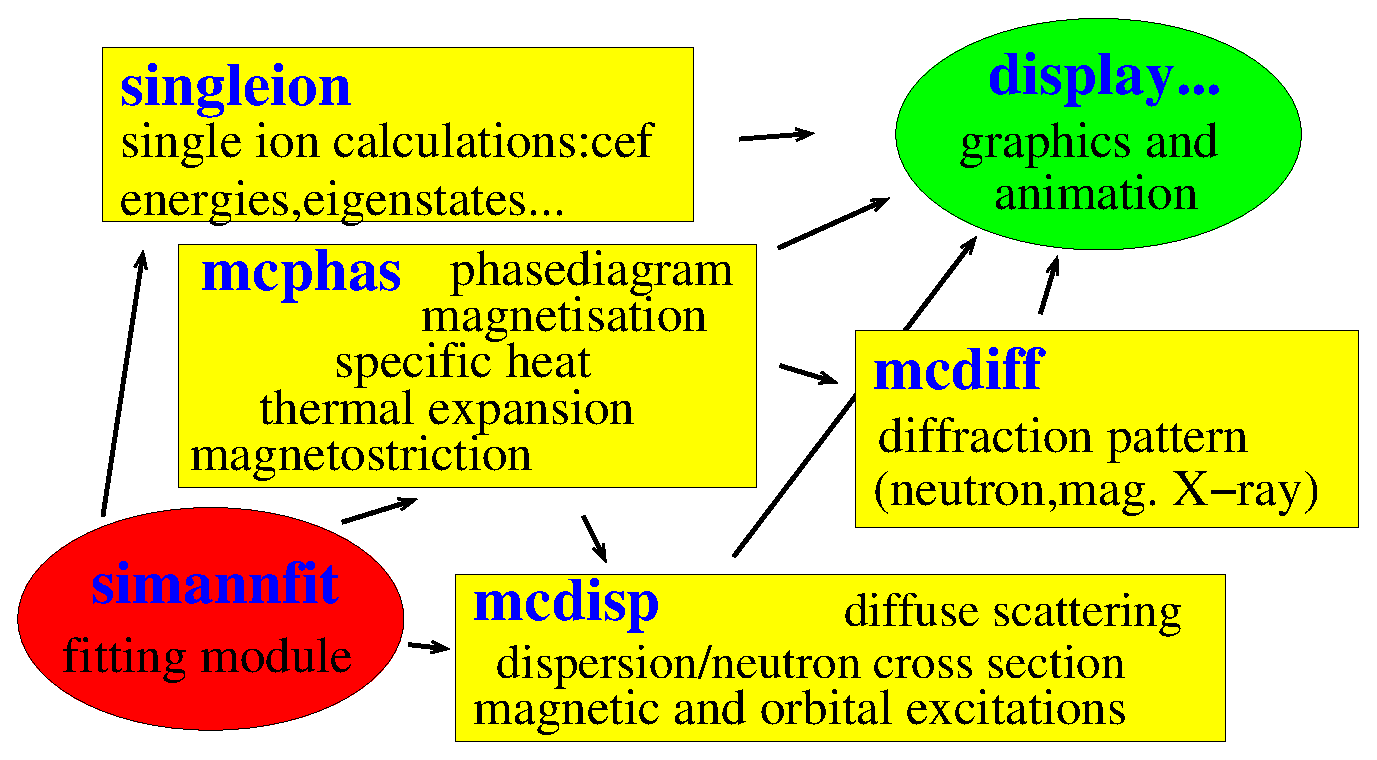
\includegraphics[angle=0,width=0.7\columnwidth]{figsrc/mcphas_modules.eps}
\caption{\label{modules}
Structure of the program package showing the tasks of the different modules.}
\end{center}
\end{figure}

\EE  For each of the many tasks of the program package separate programs have been written.
Fig.~\ref{modules} gives an overview of the 
tasks of these different modules of the program package. Have a look:
\begin{description}
\item[singleion:]
The best way to start with the program package is probably to get
acquainted with
the program {\prg singleion\index{singleion}}, which is the most important of several 
modules used for the calculation of single ion properties (see Section~\ref{cfield}).
\item[mcphas:]
This program has been written to calculate the thermodynamic properties.
In order to  deal with the pair interactions a
 combined mean-field/monte-carlo algorithm is used in module {\prg mcphas}.
For a given temperature $T$ and magnetic field $\mbf H$ (vector), electric
field and stress tensor / pressure 
 several possible magnetic structures are stabilised
by a mean field algorithm and the free energy is 
calculated. The initial values for this mean-field procedure are
modified randomly. In addition or alternatively  a Monte Carlo process according to Metropolis
stepping~\cite{metropolis53-1087} can be performed.
See Section~\ref{runmcphas} on how to perform such a simulation.


The temperature and magnetic/electric field / stress (pressure) are varied during the calculation
and thereby it is possible to map out a phase diagram.
The program produces a plot of the stabilised magnetic
structures and the magnetisation on screen, the
output files contain additional information 
such as calculated magnetoelastic and  neutron-diffraction
data. As a typical application of {\prg mcphas} the calculated magnetic
phase diagram of NdCu$_2$ is shown in fig.~\ref{ndphased}.
The exchange parameters required for the calculation of such a complex
antiferromagnet have
been determined from the dispersion of magnetic excitations
measured by neutron spectroscopy with moments aligned ferromagnetically
by an external magnetic field. Details are described elsewhere \cite{rotter00-29}.

\item[graphics:]
Several graphic programs easy the visualisation of the
calculated data (section~\ref{graphics}).

\item[mcdiff\index{mcdiff}:]
The program {\prg McDiff} can be used to calculate the magnetic neutrons
or resonant x-ray diffraction intensities. Note that neutron intensities
can be calculated going beyond the dipolar approximation for the magnetic
formfactor.

\item[mcdisp:]
An additional program {\prg McDisp} can be used to calculate the 
dispersion and intensity
 of magnetic excitations and diffuse magnetic scattering cross section.
  It is based on a mean field- random
phase approximation treatment of the problem (section~\ref{mcdisp}). 
\item[simannfit:]
In oder to enable the determination of the parameters of the
magnetic Hamiltonian from experimental data, a fitting tool
{\prg Simannfit} can be used to fit experimental  magnetic structure and excitation
data. This tool is based on the simulated annealing 
algorithm~\cite{kirkpatrick83-671} and described in section~\ref{simannfit}.
\end{description}

\begin{figure}[ht]\begin{center}
\includegraphics[angle=90,width=0.7\columnwidth]{figsrc/ndphased.eps}
\caption{\label{ndphased}
Magnetic phase diagram for NdCu$_2$ for magnetic field along
the orthorhombic $b$-direction. Colours represent the calculated phase
diagram, lines correspond to experimentally determined phase boundaries.
[plot created by program {\prg phased}]
}
\end{center}
\end{figure}


\section{Getting Started ... List of Examples}  

First some important notes .... this manual does neither give an introduction into the theory of 
magnetism nor a description of the experimental techniques. In order
to use the program successfully, some basic knowledge of crystal field theory and the mean field
approximation is required, see for instance~\cite{jensen91-1}.
In order to compare the output of the calculation with experimental
data, it is recommended to be familiar with  experimental techniques used
in the investigation of magnetic properties
such as magnetisation, susceptibility, specific heat, magnetostriction
measurements and neutron scattering.

Using {\prg McPhase} for the first time, the reader should
\begin{itemize}
\item
rush into the program and test that it functions correctly on his system
by starting the demos ( type {\prg cd demo} and then run {\prg 01\_demo\_crystal\_fields.bat},{\prg %%@
02\_demo\_mcphas\_I\_NdCu2.bat}, etc.).  In addition a complete test of
functionality can be done by typing {\prg mctest test*.bat}
\item 
learn about some special features and basic functions of the program package by
doing the tutorial in directory {\prg tutorial}
\item
look at the example calculations in directory {\prg examples}. These examples cover a large variety
of problems, which the program package may be applied to (see table~\ref{examples}). In addition, this directory
contains a large number of single ion property files which will be useful for setting
up numerical calculations for a specific system.
\item
with the help of this manual, which contains also some exercises the user is advised 
to learn about all details required to do a successful simulation of atomic magnetic properties
and set up calculations, which hopefully will be useful to interpret a large variety of 
experimental data. 
\end{itemize}

\begin{table}[thb] 
\begin{center}  
\caption {Description of the example calculations, which come along with the program package {\prg McPhase} in directory {\prg %%@
examples}:}   
\label{examples}   
\begin{tabular} 
{l|l|l|l}
name /       & problem & single ion & references \\ 
compound     &          & module  &             \\
\hline
{\prg bfk }    & Becker Fulde Keller Theorie for & {\prg so1ion }\index{bfk} &  \cite{becker77-9}, \\
               &  CF-conduction electron interaction & &  App.~\ref{bfktheory}\\
Ce3p\_chain\_cfphonon & Crystal Field Phonon int. on linear chain, & {\prg phonon } & \\
                      &   CF striction, theory paper & {\prg so1ion } & \\
Ce3p\_tetragonal\_prim & Crystal Field Phonon interaction & {\prg phonon} &  \\
                     &  on primitive lattice, CF magnetostriction & {\prg so1ion } & \\
CeAl2\_cfphonon\_cfstr &  CeAl$_2$ - Crystal Field phonon int., & {\prg phonon}, &  \\
                       &   CEF magnetostriction &   {\prg so1ion } &  \\
CeCu$_2$       & mag phase diagram, fit of dispersive  & {\prg kramer}\index{kramer} & \cite{loewenhaupt06-775,schedler03-1313} \\
               & mag. excitations to neutron data      &               & \\
CePd$_2$Si$_2$ & neutron diffraction going beyond  & {\prg %%@
so1ion}&\cite{rotter09-140405} \\
               & dipolar approx for mag. formfactor & &\\     
CoO            & magnetic formfactor - flipping ratios,   &{\prg  ic1ion} & \\
               & highly inelastic neutron scattering      &               & \\
Cu$_2$OSeO$_3$ & interacting clusters of four spins & {\prg cluster} & \cite{romhany14-xxx}\\
DyCu$_2$       & quadrupolar order and phase diagram & {\prg cfield}\index{cfield}&\cite{yoshida98-1421} \\
DyNi$_2$B$_2$C & magnetic phase diagram, special single  & {\prg %%@
quartett.so}\index{quartett.so}& \\
               & ion module (quasiquartet) &&\\
ErNi$_2$B$_2$C & magnetostriction and phase diagram & {\prg cfield}&\cite{doerr02-5609}\\
Gd$_3$GaO$_6$  & pointcharge model for crystal field parameters & {\prg pointc} & \\ 
GdNi$_2$B$_2$C & double-q magnetic structure, spin only (L=0) & {\prg brillouin}\index{brillouin}& \cite{doerr02-5609,jensen08-134408}\\
GdRu$_2$Si$_2$ & biquadratic interactions - magnetisation, mag. structure & {\prg cfield} & \\
helix\_spinwave & spinwave calculation for a helical magnetic structure & {\prg so1ion} & \\
Ho$_2$Ti$_2$O$_7$ & diffuse magnetic scattering, external stress & {\prg so1ion} & \cite{bramwell01-1495}\\
                  & cf-phonon interaction, INS, magnetostriction & {\prg phonon} & \\
LaCoO$_3$ & spin polarons quasielastic scattering & {\prg cluster}\index{cluster} & \cite{podlesnyak11-134430,podlesnyak08-247603} \\
La$_2$CoO$_4$ & dispersive magnetic excitations / spinwaves &{\prg  ic1ion} & \cite{lewtas10-184420}\\
LuMnO$_3$ &  magnetic structure and dispersion of excitations & {\prg so1ion} & \cite{lewtas10-184420} \\
NdBa$_2$Cu$_3$O$_7$ & fit of magnetic neutron diffraction  & {\prg cfield}\index{cfield} & \cite{rotter09-140405} \\
                    & data going beyond dipapprox && \\
NdCu$_2$  & crystal field, magnetic structure,  & {\prg cfield}& %%@
\cite{loewenhaupt95-491,loewenhaupt96-499,rotter00-29} \\
                    & phase diagrams with Monte Carlo, excitations &&\cite{rotter02-751,rotter02-8885} \\
NiO            & INS and RIXS on NiO & {\prg so1ion}\index{so1ion} & \\
PrNi$_2$B$_2$C & crystal field - fit to neutrons,cp, susc & {\prg cfield}&\cite{mazumdar08-144422}\\
PrNi$_2$Si$_2$ & excitons in an amplitude modulated mag structure & {\prg so1ion}\index{so1ion} & \cite{blanco13-104411} \\
Pr$_3$Pd$_{20}$Si$_6$ & hyperfine interactions & {\prg cluster}\index{cluster} & \\
PuPd$_3$ & susceptibility, heat capacity & {\prg ic1ion}\index{ic1ion} & \cite{le10-155136} \\
Ru3p\_create\_sipf & how to create paramters for a sipf file from  & {\prg simannfit,cowan} & \cite{cowan81-1} \\
                   & a Hartree Fock Calculation & {\prg RCN36K,RCN2K} & \\
TbCu$_2$ & magnetic phases with field parallel $a$ & {\prg cfield} \\
TmNiC$_2$ & determine point charge set to obey high-T exp. $B_2^0$,$B_2^2$ & {\prg so1ion,phonon}  & \\
          & with bonding e-charges.Strain,INS with cf-phonon int. &  & chap.\ref{determinePcmodel}\\
testic1ion & Pr$^{3+}$ chargedensity in IC and LS coupling & {\prg ic1ion,cfield} &\\
tungsten& phonons in tungsten & {\prg phonon} & \\
UPd$_3$ & dispersive CEF excitations, quadrupolar interactions  & {\prg so1ion}\index{so1ion} & \cite{le12-036002} \\
 \end{tabular}
\end{center}   
\end{table}




\clearpage
\section{The Hamiltonian}
\label{hamiltonian}
\EE
%script2html_begin{mcphasit} 
We assume a quantum mechanical system that can be described by the Hamiltonian
 \begin{equation}\label{hamilton}
 \hat \mathcal H=\sum_{n=1}^N \hat \mathcal H(n) -\frac{1}{2} \sum_{n,n',\alpha,\beta}
 {\mathcal J}_{\alpha\beta}(\mbf R_{n'} - \mbf R_n) \hat \mathcal I_{\alpha}^n \hat \mathcal I_{\beta}^{n'}.
 \end{equation}
The first term $\hat \mathcal H(n)$ denotes the Hamiltonian of
 a subsystem $n$
(e.g.~an ion, or cluster of ions). The second term describes a bilinear interaction 
between different subsystems
through the operators $\hat \mathcal I_{\alpha}^n$, with $\alpha = 1,2,...,m$. 
%script2html_end{mcphasit} 
The operators $\hat \mathcal H(n)$ 
and $\hat \mathcal I_{\alpha}^n$  act in the subspace $n$ of the Hilbert space, 
i.e. $[\hat \mathcal I_{\alpha}^n,\hat \mathcal I_{\alpha}^{n'}]=0$,
$[\hat \mathcal H(n),\hat \mathcal I_{\alpha}^{n'}]=0$ and $[\hat \mathcal H(n),\hat \mathcal H(n')]=0$
for $n \neq n'$\footnote{Note that these conditions are essential and put a  limit to the
applicability of the theory, for example in the case of charge transfer excitations from
one subsystem to the next.}.
For example, in the case of a Heisenberg
 exchange between magnetic ions we would identify the set of operators with
 $\alpha=1,2,3$ with the three components of the  spin: $\hat \mathcal I_1 \leftrightarrow \hat S_x, \hat \mathcal I_2 %%@
\leftrightarrow \hat S_y, \hat \mathcal I_3 \leftrightarrow \hat S_z$.

\OO Do we really need so many symbols - is there no simpler theory ? 
 
\EE Well, the beauty of the analysis which follows is that it can be applied to
almost any Hamiltonian of the form (\ref{hamilton}). And there are a lot ! 
 The analysis
of complex magnetic systems can thus be attempted by starting from a simple
form such as the Heisenberg model and by introducing, step-by-step, more
complexity into the model. For example, anisotropy and interactions with extended range can be introduced by modifying ${\mathcal J}_{\alpha\beta}(\mbf R_n - \mbf R_{n'})$, higher order operators can be 
introduced  by extending the index range for $\alpha$, and a complex single-ion term $\hat \mathcal H(n)$ may be added. 
Another example for a Hamiltonian (\ref{hamilton})  is the problem of lattice dynamics, which can
 be treated in the framework of this
formalism by identifying the operators $\hat \mathcal I^n_{\alpha}$
 with the atomic displacements $u^{n}$. Here the index $\alpha$ is not necessary and
$n$ refers to both, the atomic position index and the spatial coordinate of the displacement,
  $n=(1,x),(1,y),(1,z),(2,x),(2,y),(2,z), ...$. Note that this can be done, because the three spatial components of the 
displacement operators commute with each other (in contrast to the components of the spin) and each displacement
component acts in its own subspace of the Hilbert space. The kinetic energy
will be part of the single ion term $ \hat \mathcal H(n)$. Allowing more complexity to the system,
both the spin and lattice degrees of freedom can be introduced and spin-phonon interactions can be
handled by the theory.

\PP For the exotic matter which is todays main scientific interest because everything else is
pretty well studied, there are important limits to your approach - I guess you are aware !

\EE The main limitation of the approach is that it neglects fluctuations associated with phase 
transitions and quantum disorder. We are primarily concerned, therefore, with excitations 
associated with a  well-ordered ground state.

Two special forms of the Hamiltonian (\ref{hamilton}), which have been implemented
are given in the following. Some other forms are also available, by programming
a single ion module the user may treat any type single ion Hamiltonian $\hat \mathcal H(n)$.


\subsection{Rare Earth Ions}

\OO My sample contains rare earth - so we need to do simulations for rare earth materials.

\EE Yes, we can -
a specific example of (\ref{hamilton}) is the following magnetic  Hamiltonian $\mathcal H$ for rare earth ions,
 which may be treated with the program package:

\begin{equation}
\label{hamiltonre}
 {\mathcal H}= \sum_{n,lm} B_l^m O_{lm}({\mbf J}^n) 
             -\frac{1}{2}  \sum_{nn'} {\mathcal J}(nn') {\mbf J}^n{\mbf J}^{n'}
	     - \sum_{n} g_{Jn} \mu_B {\mbf J}^n {\mbf H} 
\end{equation}

The first term describes the crystal field (Stevens Operators $O_l^m$, see table in appendix~\ref{stevens}), the second %%@
the magnetic
exchange interaction, the third the Zeeman energy if an external magnetic field is applied.
Note that by ''external magnetic field $\mbf H$'' we refer to the magnetic field in the sample, 
which is the applied field (e.g. generated by a coil) diminished by 
the demagnetizing tensor $\m{n}_{\rm demag}$ times the magnetisation $\mbf M$ of the sample, i.e. 
$\mbf H= \mbf H_{\rm applied} - \m{n}_{\rm demag} \mbf M$, e.g. for a spherical sample $\m{n}_{\rm demag}=\m{1}/3$. 
The unit of $\mbf H$ is usually chosen to be Tesla, which actually refers to the quantity 
$\mu_0 \mbf H$ (in SI units). 

\OO I know about the demagnetisation factor, in our pulsed field experiments we sometimes
have extremely large moments and for a small sample the corrections can be quite large.

\PP I have done a lot of experiments on exotic matter, we need some other concepts than
your theory. Can you do orbital excitations ? 

\EE Instead (or rather in addition) to this it is also possible to treat the 
more general two ion exchange coupling\footnote{For further information on the notation and symmetry restrictions to the
parameters in the Hamiltonian refer to~\cite{jensen91-1}.}

\begin{equation}
\label{multipolehamilton}
 {\mathcal H}_{JJ}=
             -\frac{1}{2}  \sum_{nn'} \sum_ {ll'} \sum_{mm'}
	     {\mathcal K}_{ll'}^{mm'}(nn') O_{lm}({\mbf J}^n) O_{l'm'}({\mbf J}^{n'})
\end{equation}

\OO Well - I have magnetostriction data, we need some theoretical explanation for the strain. 
 Can you enter some magnetoelastic terms in the Hamiltonian ? I know a theoretician in Spain who has
done so and has written two huge volumes about magnetostriction. 

\EE  Indeed, in  addition to the above terms in the Hamiltonian the coupling of magnetic and lattice properties
is possible by introducing magnetoelastic interactions:
In order to calculate magnetoelastic effects the parameters 
$B_l^m$, ${\mathcal J}(ij)$ (or more general
the ${\mathcal K}_{ll'}^{mm'}(ij)$) are expanded in a Taylor expansion in the strain tensor
$\epsilon$ resulting in the magnetoelastic interaction (i.e. keeping only the terms linear
in $\epsilon$). The equilibrium strain can be 
calculated by considering in addition the elastic energy and minimising the total free energy.
\footnote{The procedure is described in detail in~\cite{rotter02-8885}.}
 
\PP If I give you a student of mine and he starts doing McPhase, are there
some exercises so he can learn how to use the program ?

\vspace{1cm}

{\em Exercises:}
\begin{itemize}
\item Write down the list of nonzero crystal field parameters in the crystal field Hamiltonian
of a Nd$^{3+}$ ion in an orthorhombic crystal field (Section~\ref{cfield} describes how such a parameter set
enters a {\prg McPhase} calculation).
\item Taking a primitive orthorhombic lattice of Nd$^{3+}$ ions write down the most general
anisotropic bilinear interaction  for the nearest neighbour exchange interaction
(Section~\ref{mcphasj} describes how such a parameters set enters a {\prg McPhase calculation}).
\end{itemize}

%The $\tilde O_l^m$ in are the Racah  operators, which form a set of irreducible
%tensor operators.

\subsection{Intermediate Coupling}

For some rare earth ions and for transition metals or actinides it is necessary to
include more singleion ion states with differen L,S into the calculation. This
can be done in intermediate coupling using the module {\prg ic1ion}\index{ic1ion}, which
explicitely includes electrostatic and  spin orbit interactions for each ion:

\begin{eqnarray}
\label{ichamilton}
 {\mathcal H}&=& \sum_n \left \{ \sum_{i_n=1}^{\nu_n}
 \left [ \frac{p_{i_n}^2}{2m_e}
        -\frac{Z_n e^2}{4\pi\epsilon_0|\mbf r_{i_n}-\mbf R_n|}
        +\zeta_n  \mbf l^{i_n} \cdot \mbf s^{i_n}
        + \sum_{lm} L_l^m(n) T_{lm}^n
\right ]
              + \sum_{i_n>j_n=1}^{\nu_n}\frac{e^2}{4\pi\epsilon_0|\mbf r_{i_n}-\mbf r_{j_n}|} \right \} \nonumber \\
	    && - \sum_{n}  \mu_B (2\mbf S^n+\mbf L^n) {\mbf H}  \nonumber\\
            && -\frac{1}{2} \sum_{nn'} \left[ 
({\hat \mbf S}^n,{\hat \mbf L}^n )
\stackrel{=}{\mathcal J}(nn') 
\left ( \begin{array}{c} {\hat \mbf S}^{n'} \\
        {\hat \mbf L}^{n'} \end{array}
\right )
     + \sum_{kk'} \sum_{qq'}  \mathcal{K}_{kk'}^{qq'}(nn') \hat{T}_{kq}^n T_{k'q'}^{n'} \right]
\end{eqnarray}

Here $\nu_n$,$Z_n$ and $\mbf R_n$ denote the number of electrons, the charge of the nucleus
and the position
 of the ion number $n$,respectively, for each electron being
$p$ the momentum, $m_e$ the mass, $e$ the charge and $\mbf r$ the location.
Spin orbit coupling is written in terms of the orbital momentum $\mbf l$ and
spin $\mbf s$ of the individual electrons. The
 Zeman interaction and two ion interaction are written in terms of 
the (inverse) total spin $\mbf S_n$ and (inverse) total orbital momentum $\mbf L_n$
of ion number $n$. The crystal field in intermediate coupling is written
in terms of Wybourne parameters $L_l^m$ and Wybourne operators $T_{lm}^n$, operator equivalents
of real valued 
spherical harmonic functions 
$T_{l0}=\sqrt{4\pi/(2l+1)}\sum_iY_{l0}(\Omega_{i_n})$, 
$T_{l,\pm|m|}=\sqrt{4\pi/(2l+1)}\sum_i \sqrt{\pm1}[Y_{l,-|m|}(\Omega_{i_n})\pm (-1)^m Y_{l,|m|}(\Omega_{i_n})]$ for the ion $n$,
for details on crystal field parameter 
conventions see appendix~\ref{cfparconventions}.

\clearpage
{\small
\subsection{Summary}

The Hamiltonian is in general:
\begin{equation}
    \hat{\mathcal{H}}
    =
    \sum_{n=1}^{N}
    \hat{\mathcal{H}}(n)
    -
    \frac{1}{2}
    \sum_{n,n^{\prime},\alpha,\beta}
    \mathcal{J}_{\alpha,\beta}(\mathbf{R}_{n^{\prime}} - \mathbf{R}_{n})
    \hat{\mathcal{I}}_{\alpha}^n
    \hat{\mathcal{I}}_{\beta}^{n^{\prime}}
\end{equation}

The first term $\hat{\mathcal{H}}(n)$ denotes the Hamiltonian of a
subsystem $n$ (e.~g. an ion, or cluster of ions). The second term
describes a bilinear interaction between different subsystems through the
operators $\hat{\mathcal{I}}_{\alpha}^n$, with $\alpha = 1, 2, \dots, m$.
The operators $\hat{\mathcal{H}}(n)$ and $\hat{\mathcal{I}}_{\alpha}^n$
act in the subspace $n$ of the Hilbert space, i.~e. 
$[\hat{\mathcal{I}}_{\alpha}^n, \hat{\mathcal{I}}_{\alpha}^{n^{\prime}}] = 0$,
$[\hat{\mathcal{H}}(n), \hat{\mathcal{I}}_{\alpha}^{n^{\prime}}] = 0$
and
$[\hat{\mathcal{H}}(n), \hat{\mathcal{H}}(n^{\prime})] = 0$
for $n \ne n^{\prime}$.

Next we give specific examples which fill the above expression with life.


\subsubsection{Zeeman energy}

When an external magnetic field is applied the term of the form 
\begin{equation}
    \hat{\mathcal{H}}_{Z-J}(n)
    =
    -
    \sum_{\alpha=1,2,3}
    g_n
    \mu_B
    \hat{J}^{n}_{\alpha}
    H_{\alpha}
\end{equation}
where $\hat{\mathbf{J}}^n$ is a total angular momentum operator, is included.

Or the term of the form
\begin{equation}
    \hat{\mathcal{H}}_{Z-LS}(n)
    =
    -
    \sum_{\alpha=1,2,3}
    \mu_B
    \Bigl(
        2 \hat{S}^n_{\alpha} + \hat{L}^n_{\alpha}
    \Bigr)
    H_{\alpha}
\end{equation}
where $\hat{\mathbf{S}}^n$ and $\hat{\mathbf{L}}^n$ are the (inverse)
spin and orbital angular momentum operators of the ion $n$, respectively.

Note that by "external magnetic field $\mathbf{H}$" we refer to the
magnetic field in the sample, which is the applied field (e.~g. generated by a
coil) diminished by the demagnetizing tensor $\overline{n}_{\text{demag}}$
times the magnetisation $\mathbf{M}$ of the sample, i.~e.
$\mathbf{H} = \mathbf{H}_{\text{applied}} - \overline{n}_{\text{demag}} \mathbf{M}$,
e.~g. for a spherical sample $\overline{n}_{\text{demag}} = 1/3\,\overline{I}$,
where $\overline{I}$ is the identity matrix. The unit of $\mathbf{H}$
is usually chosen to be Tesla, which actually refers to the quantity
$\mu_0 \mathbf{H}$ (in SI units).

\subsubsection{Magnetic exchange}

Isotropic magnetic exchange interaction (e.~g. Heisenberg exchange) is written as
\begin{equation}
    \hat{\mathcal{H}}_{X-J}
    =
    -
    \frac{1}{2}
    \sum_{nn^{\prime}, \alpha\beta=1,2,3}
    \mathcal{J}(\mathbf{R}_{n^{\prime}} - \mathbf{R}_{n})
    \hat{\mathcal{I}}_{\alpha}^n
    \hat{\mathcal{I}}_{\beta}^{n^{\prime}}
\end{equation}
where the operators are understood as
$\hat{\mathcal{I}}_{1}  \leftrightarrow \hat{J}_x$,
$\hat{\mathcal{I}}_{2}  \leftrightarrow \hat{J}_y$,
$\hat{\mathcal{I}}_{3}  \leftrightarrow \hat{J}_z$.

\subsubsection{Intermediate coupling}

For some rare earth ions and for transition metals or actinides it is necessary
to include more single-ion ion states with different L, S into the calculation.
Two-ion intermediate interaction can be written as 
\begin{equation}
    \hat{\mathcal{H}}_{IC}
    =
    -
    \frac{1}{2}
    \sum_{nn^{\prime},\alpha\beta=1,\dots,6}
    \mathcal{J}_{\alpha\beta}(\mathbf{R}_{n^{\prime}} - \mathbf{R}_{n})
    \hat{\mathcal{I}}_{\alpha}^n
    \hat{\mathcal{I}}_{\beta}^{n^{\prime}}
\end{equation}
where the operators are understood as
$\hat{\mathcal{I}}_{1}  \leftrightarrow \hat{S}_x$,
$\hat{\mathcal{I}}_{2}  \leftrightarrow \hat{S}_y$,
$\hat{\mathcal{I}}_{3}  \leftrightarrow \hat{S}_z$,
$\hat{\mathcal{I}}_{4}  \leftrightarrow \hat{L}_x$,
$\hat{\mathcal{I}}_{5}  \leftrightarrow \hat{L}_y$,
$\hat{\mathcal{I}}_{6}  \leftrightarrow \hat{L}_z$.

\subsubsection{Dzyaloshinskii-Moriya interaction}

DMI can be written in the form of the two-ion interaction as
\begin{equation}
    \hat{\mathcal{H}}_{DMI}
    =
    -
    \frac{1}{2}
    \sum_{nn^{\prime},\alpha\beta=1,2,3}
    \mathcal{J}_{\alpha\beta}(\mathbf{R}_{n^{\prime}} - \mathbf{R}_{n})
    \hat{\mathcal{I}}_{\alpha}^n
    \hat{\mathcal{I}}_{\beta}^{n^{\prime}}
\end{equation}
where the operators are understood as
$\hat{\mathcal{I}}_{1}  \leftrightarrow \hat{J}_x$,
$\hat{\mathcal{I}}_{2}  \leftrightarrow \hat{J}_y$,
$\hat{\mathcal{I}}_{3}  \leftrightarrow \hat{J}_z$ and
$\mathcal{J}_{\alpha\beta}(\mathbf{R}_{n^{\prime}} - \mathbf{R}_{n})$ is a
skew-symmetric matrix.

\subsubsection{Classical dipole dipole interaction}

Classical magnetic dipole-dipole interaction can be written in the form of the
two-ion interaction with the matrix parameter 
\begin{equation}
    \hat{\mathcal{H}}_{CDD}
    =
    -
    \frac{1}{2}
    \sum_{n\ne n^{\prime},\alpha\beta=1,2,3}
    \mathcal{J}_{\alpha\beta}(\mathbf{R}_{n^{\prime}} - \mathbf{R}_{n})
    \hat{\mathcal{I}}_{\alpha}^n
    \hat{\mathcal{I}}_{\beta}^{n^{\prime}}
\end{equation}
where the operators are understood as
$\hat{\mathcal{I}}_{1}  \leftrightarrow \hat{J}_x$,
$\hat{\mathcal{I}}_{2}  \leftrightarrow \hat{J}_y$,
$\hat{\mathcal{I}}_{3}  \leftrightarrow \hat{J}_z$ and 
\begin{equation}
    \mathcal{J}_{\alpha\beta}(\mathbf{R}_{n^{\prime}} - \mathbf{R}_{n})
    =
    \frac{\mu_0\mu_B^2 g_n g_{n^{\prime}}}{2\pi}
    \Biggl(
        3\frac{(R_{n^{\prime}}^{\alpha} - R_{n}^{\alpha})(R_{n^{\prime}}^{\beta} - R_{n}^{\beta})}{|\mathbf{R}_{n^{\prime}} - \mathbf{R}_{n}|^5}
        -
        \frac{\delta_{\alpha\beta}}{|\mathbf{R}_{n^{\prime}} - \mathbf{R}_{n}|^3}
    \Biggr)
\end{equation}

\subsubsection{Crystal field}

Single-ion crystal field is written with Stevens operators as
\begin{equation}
    \hat{\mathcal{H}}_{CF1-S}(n)
    =
    \sum_{lm}
    B_l^m
    \hat{O}_{lm}(\mathbf{J}^n)
\end{equation}
or with Wybourne operators $\hat{T}_{lm}^n$ and Wybourne parameters
$L_l^m$ as
\begin{equation}
    \hat{\mathcal{H}}_{CF1-W}(n)
    =  
    \sum_{lm}
    L_l^m(n)
    \hat{T}_{lm}^{n}
\end{equation}
where $\hat{T}_{lm}^n$ is an operator equivalents of real valued spherical
harmonic functions
\begin{eqnarray}
    \hat{T}_{l0}
    &=&
    \sqrt{4\pi/(2l+1)}
    \sum_i
    Y_{l0}(\Omega_{i_n}),
    \nonumber\\
    \hat{T}_{l,\pm|m|}
    &=&
    \sqrt{4\pi/(2l+1)}
    \sum_i
    \sqrt{\pm 1}
    [Y_{l,-|m|}(\Omega_{i_n}) \pm (-1)^m Y_{l,|m|}(\Omega_{i_n})]
\end{eqnarray}
for the ion $n$, where index $i_n$ runs over all electrons in the
open shell of an ion (d, f). Two-ion crystal field can be written with the
Stevens operators as
\begin{equation}
    \hat{\mathcal{H}}_{CF2-S}
    =
    -\frac{1}{2}
    \sum_{nn^{\prime}}
    \sum_{ll^{\prime}}
    \sum_{mm^{\prime}}
    K_{ll^{\prime}}^{mm^{\prime}}(nn^{\prime})
    \hat{O}_{lm}(\mathbf{J}^n)
    \hat{O}_{l^{\prime}m^{\prime}}(\mathbf{J}^{n^{\prime}})
\end{equation}
or with the Wybourne operators  as
\begin{equation}
    \hat{\mathcal{H}}_{CF2-W}
    =
    -
    \frac{1}{2}
    \sum_{nn^{\prime}}
    \Biggl[
        \sum_{kk^{\prime}}
        \sum_{qq^{\prime}}
        \mathcal{K}_{kk^{\prime}}^{qq^{\prime}}(nn^{\prime})
        \hat{T}_{kq}^n
        \hat{T}_{k^{\prime}q^{\prime}}^{n^{\prime}}
    \Biggr]
\end{equation}
where operators are defined as $\hat{\mathcal{I}}_{\alpha}^n \leftrightarrow \hat{O}_{lm}(\mathbf{J}^n)$
or $\hat{\mathcal{I}}_{\alpha}^n \leftrightarrow \hat{T}_{kq}^n$ and 
index $\alpha$ runs over $m$ pairs of $(l,m)$ or $(k,q)$
respectively. Interaction parameters are either
$\mathcal{J}_{\alpha,\beta}(\mathbf{R}_{n^{\prime}} - \mathbf{R}_{n}) \leftrightarrow K_{ll^{\prime}}^{mm^{\prime}}(nn^{\prime})$
or
$\mathcal{J}_{\alpha,\beta}(\mathbf{R}_{n^{\prime}} - \mathbf{R}_{n}) \leftrightarrow \mathcal{K}_{kk^{\prime}}^{qq^{\prime}}(nn^{\prime})$,
where index $\beta$ runs over $m$ pairs of $(l^{\prime},m^{\prime})$ or $(k^{\prime},q^{\prime})$
respectively.


\subsubsection{Exchange striction}

\begin{equation}
    \hat{\mathcal{H}}_{XS}
    =
    -
    \frac{1}{2}
    \sum_{\stackrel{nn^{\prime},\alpha\beta\alpha^{\prime}\gamma=1,2,3}{beta^{\prime}=1-6}}
    \Biggl(
        \frac{\partial \mathcal{J}_{\alpha\beta}}{\partial \epsilon_{\beta^{\prime}}}
        +
        \frac{\partial \mathcal{J}_{\alpha\beta}}{\partial R_{nn^{\prime}}^{\alpha^{\prime}}}
        \frac{\partial \epsilon_{\alpha^{\prime}\gamma} R_{nn^{\prime}}^{\gamma}}{\partial \epsilon_{\beta^{\prime}}}
    \Biggr)
    \epsilon_{\beta^{\prime}}
    \hat{\mathcal{I}}_{\alpha}^n
    \hat{\mathcal{I}}_{\beta}^{n^{\prime}}
\end{equation}


\subsubsection{Phonons}

A three dimensional Einstein oscillator (for atom $n$) in a solid can be
described by the following Hamiltonian
\begin{equation}
    \hat{\mathcal{H}}_{P1}(n)
    =
    \frac{a_0^2\hat{\mathbf{w}}_n^2}{2m_n}
    -
    \frac{1}{2}
    \sum_{\alpha\beta=1,2,3}
    \hat{u}_{\alpha}^n
    K(nn)
    \hat{u}_{\beta}^n
    -
    \sum_{\alpha=1,2,3}
    F_{\alpha}(n)
    \hat{u}_{\alpha}^n
\end{equation}

Here $\hat{\mathbf{u}}$ is the dimensionless displacement vector 
$\hat{\mathbf{u}} = \hat{\mathbf{P}}_n / a_0 = \Delta \hat{\mathbf{r}}_n / a_0$,
with the Bohr radius $a_0 = 0.5219$ Angstrom), $m_n$ the mass of the atom
$n$, $\hat{\mathbf{w}}_n = d\hat{\mathbf{u}}_n/dt = \mathbf{p}_n / a_0$
the conjugate momentum to $\hat{\mathbf{u}}_n$ and $\overline{K}(nn)$
the matrix describing the restoring force.

External force $\mathbf{F}(n)$ can correspond to the electric field
$\mathbf{E}_{\text{el}}$, i.~e. $\mathbf{F}(n) = q_n \mathbf{E}_{\text{el}} a_0$,
where Bohr radius $a_0$ is included in order to yield
$\mathbf{F}_{\text{el}}(n)$ in units of meV.

Coupling such oscillators leads to the Hamiltonian
\begin{equation}
    \hat{\mathcal{H}}_{P2}
    =
    -
    \frac{1}{2}
    \sum_{n\ne n^{\prime},\alpha\beta=1,2,3}
    \hat{u}_{\alpha}^n
    K_{\alpha\beta}(nn^{\prime})
    \hat{u}_{\beta}^{n^{\prime}}
\end{equation}
where operators are defined as $\hat{\mathcal{I}}_{\alpha}^n \leftrightarrow \hat{\mathbf{u}}^n_{\alpha}$
and interaction parameters are
$\mathcal{J}_{\alpha,\beta}(\mathbf{R}_{n^{\prime}} - \mathbf{R}_{n}) \leftrightarrow K_{\alpha\beta}(nn^{\prime})$.



\subsubsection{Single-ion electrostatic and spin-orbit interaction}

\begin{equation}
    \hat{\mathcal{H}}_{E-SO}(n)
    =
    \sum_{i_n=1}^{\nu_n}
    \Biggl[
        \frac{(p_{i_n})^2}{2m_e}
        -
        \frac{Z_n e^2}{4\pi \epsilon_0 |\mathbf{r}_{i_n} - \mathbf{R}_n|}
        +
        \zeta_n
        \mathbf{l}^{i_n}
        \cdot
        \mathbf{s}^{i_n}
    \Biggr]
    +
    \sum_{i_n > j_n=1}^{\nu_n}
    \frac{e^2}{4\pi \epsilon_0 |\mathbf{r}_{i_n} - \mathbf{r}_{j_n}|}
\end{equation}

Here $\nu_n,Z_n$ and $\mathbf{R}_n$ denote the number of electrons,
the charge of the nucleus and the position of the ion number $n$,
respectively, for each electron being $p$ the momentum, $m_e$
the mass, $e$ the charge and $\mathbf{r}$ the location. Spin orbit
coupling is written in terms of the orbital momentum $\mathbf{l}$ and spin
$\mathbf{s}$ of the individual electrons. 

\subsubsection{Magneto-elastic interaction}

\begin{equation}
    \hat{\mathcal{H}}_{ME1}(n)
    =
    -
    \sum_{\stackrel{\alpha=1,\dots,6,}{gamma=1,2,3}}
    G^{\alpha\gamma}_{\text{mix}}(n)
    \epsilon_{\alpha}
    \hat{u}_n^{\gamma}
    -
    \sum_{\alpha=1,\dots,6, lm}
    G^{\alpha\gamma}_{\text{cfph}}(n)
    \epsilon_{\alpha}
    O_{lm}(\hat{\mathbf{J}}^n)
\end{equation}
and 
\begin{equation}
    \hat{\mathcal{H}}_{ME2}
    =
    -
    \sum_{\stackrel{n<n^{\prime},lm,}{alpha=1,2,3}}
    \Gamma^{\alpha\gamma}(nn^{\prime})
    \hat{u}_n^{\alpha}
    O_{lm}(\hat{\mathbf{J}}^{n^{\prime}})
\end{equation}

\subsubsection{Elastic energy and external stress}

Classical elastic energy and external stress can be included as
\begin{equation}
    \hat{H}
    =
    \frac{1}{2}
    \sum_{\alpha\gamma=1-6}
    c^{\alpha\gamma}
    \epsilon_{\alpha}
    \epsilon_{\gamma}
    -
    \sum_{\alpha=1,\dots,6}
    \sigma_{\alpha}
    \epsilon_{\alpha}
\end{equation}
}
\clearpage

\input{singleion.tex}

\clearpage

\input{mcphas.tex}

\clearpage

\input{mcdiff.tex}

\clearpage

\input{mcdisp.tex}

\clearpage

\input{q_int.tex}

\clearpage

\input{phonon.tex}

\input{extsimod.tex}

\input{ic1ion.tex}
\clearpage

\input{bfk.tex}

\input{graphic_display.tex}

\clearpage

\input{fitting.tex}

\clearpage

\input{additional_programs.tex}

\clearpage		     

\appendix


\input{kramers.tex}
\input{brillouin.tex}
\input{dyni2b2c.tex}
\input{erni2b2c.tex}
\clearpage
\input{cfparconventions.tex}
\input{tesseral.tex}
\clearpage
\input{stevens.tex}
\input{cfparsymmetrytable.tex}
\input{rotateBlm.tex}

\clearpage
\input{ffacts.tex}
\input{zk.tex}
\input{cdoperator.tex}
\input{mcdisp_formalism.tex}
\input{bfktheory.tex}
\clearpage
\section{Solution of the exercises}

\begin{description}
\item[section~\ref{hamiltonian} {\em The Hamiltonian}] \ 
 \begin{enumerate}
 \item Fast and simple: take some book on crystal fields~\cite{hutchings64-227} and look up which parameters are nonzero 
 for the orthorhombic crystal field ($B_2^0$,$B_2^2$,$B_4^0$,$B_4^2$,$B_4^4$,$B_6^0$,$B_6^2$,$B_6^4$,$B_6^6$).

 Detailed Calculation: take the point group $D_2^h$, the Stevens Operators $O_l^m$ taken as a vector form
 a representation of this point group, which is reducible. Follow the procedure outlined in the book~\cite{elliott79-1}
 to split this representation into irreducible parts. The basis vectors of the unit representation may then be 
 linear combined with some arbitrary crystal field parameters to give the most general crystal field.
 Note that the basis vectors of the unit representation can be obtained efficiently by constructing the
 projection operator (eq. 4.51 in~\cite{elliott79-1})
  into the subspace transforming according to the irreducible unit representation. 
 \item Unfortunately no table is available for all relevant problems. Some cases are given in~\cite{morin90-1}.
 2 ways are possible to solve the problem. The accurate group theoretical approach which follows the calculation
 outlined above for the crystal field  and needs a lot of knowledge in group theory. However a more intuitive %%@
calculation
 can be made by writing down the most general two ion interaction and subsequent introduction of symmetry elements which
 will then give relation between parameters. As an example in the primitive orthorhombic lattice there are 2 nearest %%@
neighbours, which
 are equivalent. 

 In general the bilinear two ion interaction  has the form 
 $-\frac{1}{2}  \sum_{ij}  {\mbf J}_i^{alpha}{\mathcal J}_{\alpha\beta}(ij){\mbf J}_j^{\beta}$.
 $i$ and $j$ number the different positions of the magnetic ions in the lattice. Without loss of 
 generality the interaction constants ${\mathcal J}_{\alpha\beta}(ij)$ can be chosen such that
 ${\mathcal J}_{\alpha\beta}(ij)={\mathcal J}_{\beta\alpha}(ji)$ (because the expression is symmetric in
 angular momentum components any anisotropic part of the interaction tensor does not contribute to the
 interaction energy).  

 If $i$ and $j$ are nearest neighbours on a orthorhombic lattice, they are situated on one of the
 crystallographic axes, for example at [$\pm$100]. The off-diagonal components of the corresponding
 interaction tensor ${\mathcal J}_{\alpha\beta}(\pm100)$ vanish, because spin-configurations such as
 a moment (m00) on [000] and (0m0) on [100] must have the same magnetic energy as (m00) on [000] and
 (0-m0) on [100]. Furthermore the spin-configuration with (m00) on [000] and (m'00) on [100] must
 have the same magnetic energy as (m00) on [000] and (m'00) on [-100]. This and similar
 considerations lead to the conclusion that the interaction tensor must be the same for [-100] and
 [+100]. Therefore the most general form of the interaction ${\mathcal J}_{\alpha\beta}(\pm100)$
 is 
 \begin{equation}
 {\mathcal J}_{\alpha\beta}(\pm100)=\left(
 \begin{array}{ccc}
 {\mathcal J}_{aa}(\pm100) & 0 & 0 \\
 0 & {\mathcal J}_{bb}(\pm100) &  0 \\
 0 & 0 & {\mathcal J}_{cc}(\pm100) \\
 \end{array}
 \right)
 \end{equation}
 \end{enumerate}
\item[section~\ref{cfieldsep} {\em Using {\prg so1ion} separately}] \ 
 \begin{itemize}
 \item type: so1ion -c -B m m Nd3+ 2 10 rk
 \item edit file bkq.parameter and enter the crystal field parameters given in section~\ref{cf1ion}
 \item type: so1ion -r -B
 \item edit file results/so1ion.output to see the result of the calculation
 \end{itemize}
\item[section~\ref{start} {\em starting a simulation}] \ 

 \begin{enumerate}
 \item In the crystallographic basis there are two ions.
 \item ... the simulation should run after typing {\prg mcphas}
 \end{enumerate}
\item[section~\ref{outputfiles} {\em output files}] \ 
 \begin{enumerate}
 \item at 2.8 Tesla
 \item (0.6 0 0), (2/3 0 0) and (0.625 0 0)
 \end{enumerate}
\item[section~\ref{mcdisp} {\em {\prg McDisp} - the calculation program for magnetic excitations}] \ \\
 the inspection of the file {\prg mcdisp.mf\index{mcdisp.mf}} shows that the calculation is performed at 3.2 Tesla field
 parallel to $b$, i.e. in the ferromagnetically aligned state. Due to the two ions in the crystallographic
 unit cell in general 2 modes are expected for each crystal field transition. After running {\prg mcdisp\index{mcdisp}}
 the results may be inspected in file {\prg ./results/mcdisp.qom}, graphically using the program {\prg disp}.
 It turns out the the soft mode (gap at (2/3\,1\,0) shows the largest intensity.
\end{description}


\clearpage
\section{Unit Conventions in McPhase}

In most cases units of input parameters and output properties in {\prg McPhase} cannot be modified and 
are fixed in the program code. In output files usually the unit is given in the column header.
In table (\ref{units}) the unit conventions are listed.

\begin{table}[thb] 
\begin{center}  
\caption {Units in the program package 
{\prg McPhase}:}   
\label{units}   
\begin{tabular} 
{l|l|l|l}
Physical Quantity  & symbol                                         & unit      & typical file(s)/programs     \\
\hline
Born van Karman spring & $c_L(ij)$                                  &  N/m      &   bvk\_parameter.table  \\
Charge             &  CHARGE                                        & $|e|$     & *.sipf \\
Coupling constants & $K_{\alpha\beta}(ij)$                          & meV       & mcphas.j     \\
Crystal field parameters & $B_l^m, L_l^m$			    & meV	& *.sipf \\
Debye Waller Factor & DWF, $B_{iso}/2$                              & \AA$^2$   & *.sipf, mcdiff.in \\ 
Phonon-Displacement	   & $\mbf P$                               & \AA       & singleion, spins   \\
Phonon-Displacement	   & $\mbf u$                               & 1         & singleion   \\
Electric Field	   & $\mbf E_{\rm el}$				    & kV/mm     & mcphas.ini, mcphas.fum \\
Electric Polarisation & $\mbf P_{\rm el}$			    & |e|/\AA$^2$ & mcphas.fum \\
Elastic constants  &  $c^{\alpha\beta} $			    & meV/primitve unit cell & mcphas.j \\
Elastic Energy     &  $E_{elastic}$				    & meV/ion	& mcphas.fum \\
Energy             & cf-parameters Blm Llm, free energy u           & meV       & *.sipf, mcphas.fum ...  \\
Lattice Constant   & a,b,c                                          & \AA        & mcdiff.in, mcphas.j \\
Magnetic Field     & H, Ha, Hb, Hc                                  & Tesla     & mcphas.ini, mcdisp.mf ...    \\
Magnetic Moment    &  mu, $\mu$                                     & $\mu_B$   & mcphas.fum \\
Neutron Cross Section &  sigma ,$\sigma$                            & barn      & mcdisp.qei \\
Neutron Scattering Length & SCATTERINGLENGTHREAL & $10^{-12}$~cm & *.sipf, mcdiff.in \\
  & SCATTERINGLENGTHIMAG & & \\
Radial Integrals   & R2,R4,R6 , $\langle r^l \rangle$               & $a_0^2$, $a0=0.5292$~\AA \\ 
Stress tensor	   & $\sigma^{\alpha}$				    & GPa	& mcphas.fum, mcphas.ini \\
Temperature        & T                                              & Kelvin    & mcphas.ini, mcdisp.mf ... \\
Wave length        & lambda, $\lambda$                              & \AA       & mcdiff.in \\
Wave vector        & k, ki, kf, Q, Qx, Qy, Qz                       & 1/\AA    & mcdisp.par \\

\end{tabular}
\end{center}
\end{table}

\clearpage
\section{Installation of the program package}

\input{../install.txt}


\newpage

\bibliographystyle{physrev}   % here you should update any list by
\bibliography{li120914}   % bibtex - ing the database

\newpage
\printindex
\input{shortlist.tex}
\end{document}
